\chapter{Implementation}
\label{ch:implementation}

\todo{Write chapter introduction}

\section{Chauffeur Service}

%  \begin{itemize}
%     \item Take some Pictures
%     \item Chauffeur service for German federal agency.
%     \item Takes new Chauffeur Jobs
%     \item UI overview of Jobs, and Jobs Details
%     \item Overview of Chauffeurs and their availability 
%     \item UI to manage Jobs, assign chauffeurs
%     \item group Jobs
%  \end{itemize}

As a basis for our case study we used an application called DSW-FD (Dispositions-software-Fahrdienst). DSW-FD is used to schedule chauffeur rides for a German federal agency. The application provides a rich user interface with views for managing chauffeur jobs, as well as chauffeur drivers. Clients which need a Chauffeur ride can call a separate hotline, where a handler creates a new chauffeur job, this job is then sent to DSW-FD where it appears in the overview of Jobs and can then be processed by a Job handler.

Drivers need to be manually assigned to a job by a handling person. To this end, the application provides suggestions for drivers which would be free when the job is schedule and are closest to the job's departure point. Furthermore, the app provides functionality to group together different jobs so that they may be handled by a single driver, determine the return destination for the driver after they finished the job, as well as marking a job as being handled by a pool of drivers.

The application also provides features to directly interact with drivers, such as broadcasting messages to all drivers, reminding a driver to take their mandatory break, and directly calling a driver.

\section{Current Implementation}

% \begin{itemize}
%     \item UI5-Frontend
%     \item Java-Backend
%     \item Android app for drivers.
%     \item OIDC
%     \item mssql
% \end{itemize}

The current Implementation is realized as a classic frontend, backend architecture. The backend is implemented using the Java web framework Spring\footnote{\url{https://spring.io/}}. It provides a SOAP web server on which new Jobs are submitted from another service. Data is persisted in a MSSQL database. The backend also provides Multiple REST API's and an OData API for communication with the frontend. Furthermore, the backend has to interact with Firebase to trigger push notifications on smartphone devices.

The System provides two frontends, an android application, which is used by the chauffeur drivers to receive jobs and communication from headquarters and a web client which is used by handlers to manage jobs and drivers. The web client is implemented using OpenUI5\footnote{\url{https://openui5.org/}}. OpenUI5 is a frontend framework published by SAP, it is intended for development of enterprise applications which follow SAP's Fiori design guidelines\footnote{\url{https://experience.sap.com/fiori-design/}}. All APIs of the backend require authentication. To this end the frontend has to authenticate with a Keycloak\footnote{\url{https://www.keycloak.org/}} instance using OpenID Connect (OIDC). An overview of the system architecture is provided in \Cref{fig:dswfd-architecture}.

\begin{figure}[ht]
    \centering
    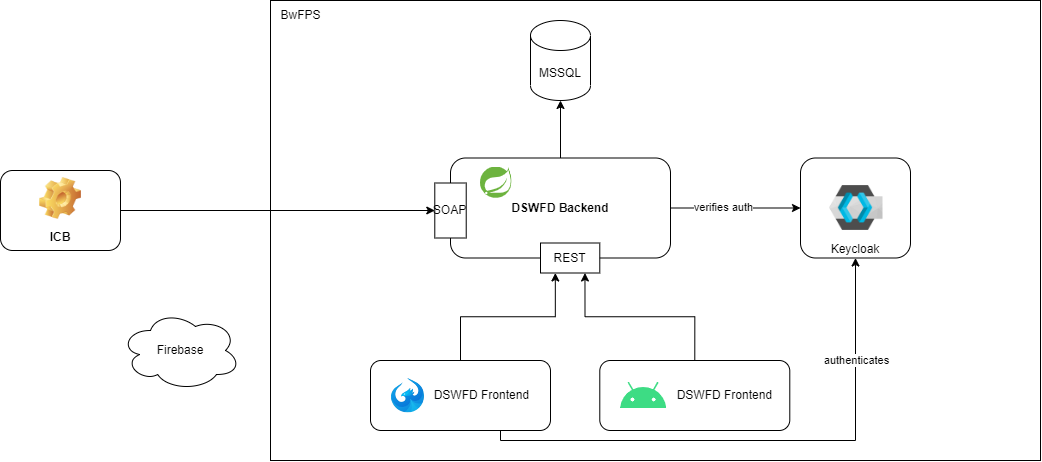
\includegraphics[width=.8\linewidth]{assets/dswfd-architecture}
    \caption{Architecture overview of the current implementation}
    \label{fig:dswfd-architecture}
\end{figure}

\section{SvelteKit Implementation}

% \begin{itemize}
%     \item Two approaches (full stack, FE only)
%     \item First try UI5 web components, second try CSS classes
%     \item Authentication
% \end{itemize}

Our study focused on the core of DSW-FD's system landscape, comprised of the Spring backend and the OpenUI5 web frontend. We experimented with two different implementations. One where SvelteKit replaces both the backend and frontend and one where SvelteKit only replaces the frontend. Both our implementations had to communicate with the Keycloak service to authenticate. The full stack implementation also had to interact with the MSSQL database. As to not widen the scope too much, API's for the android application, Firebase communication, and the SOAP API for ICB was not implemented. We also decided to use TypeScript instead of regular JavaScript. This provided a better developer experience with little extra overhead. Because SvelteKit can infer types for most of its internal functionality. Extra types had to be only defined for external API's.

We focused our implementation on a subset of features required to manage chauffeur jobs. To this end we implemented three pages. The overview page that shows all currently relevant chauffeur jobs (\Cref{fig:current-overview-auftrag}). The detail page for chauffeur jobs (\Cref{fig:current-details-auftrag}). And a view that is used to create new (internal) chauffeur jobs.

\begin{figure}
    \centering
    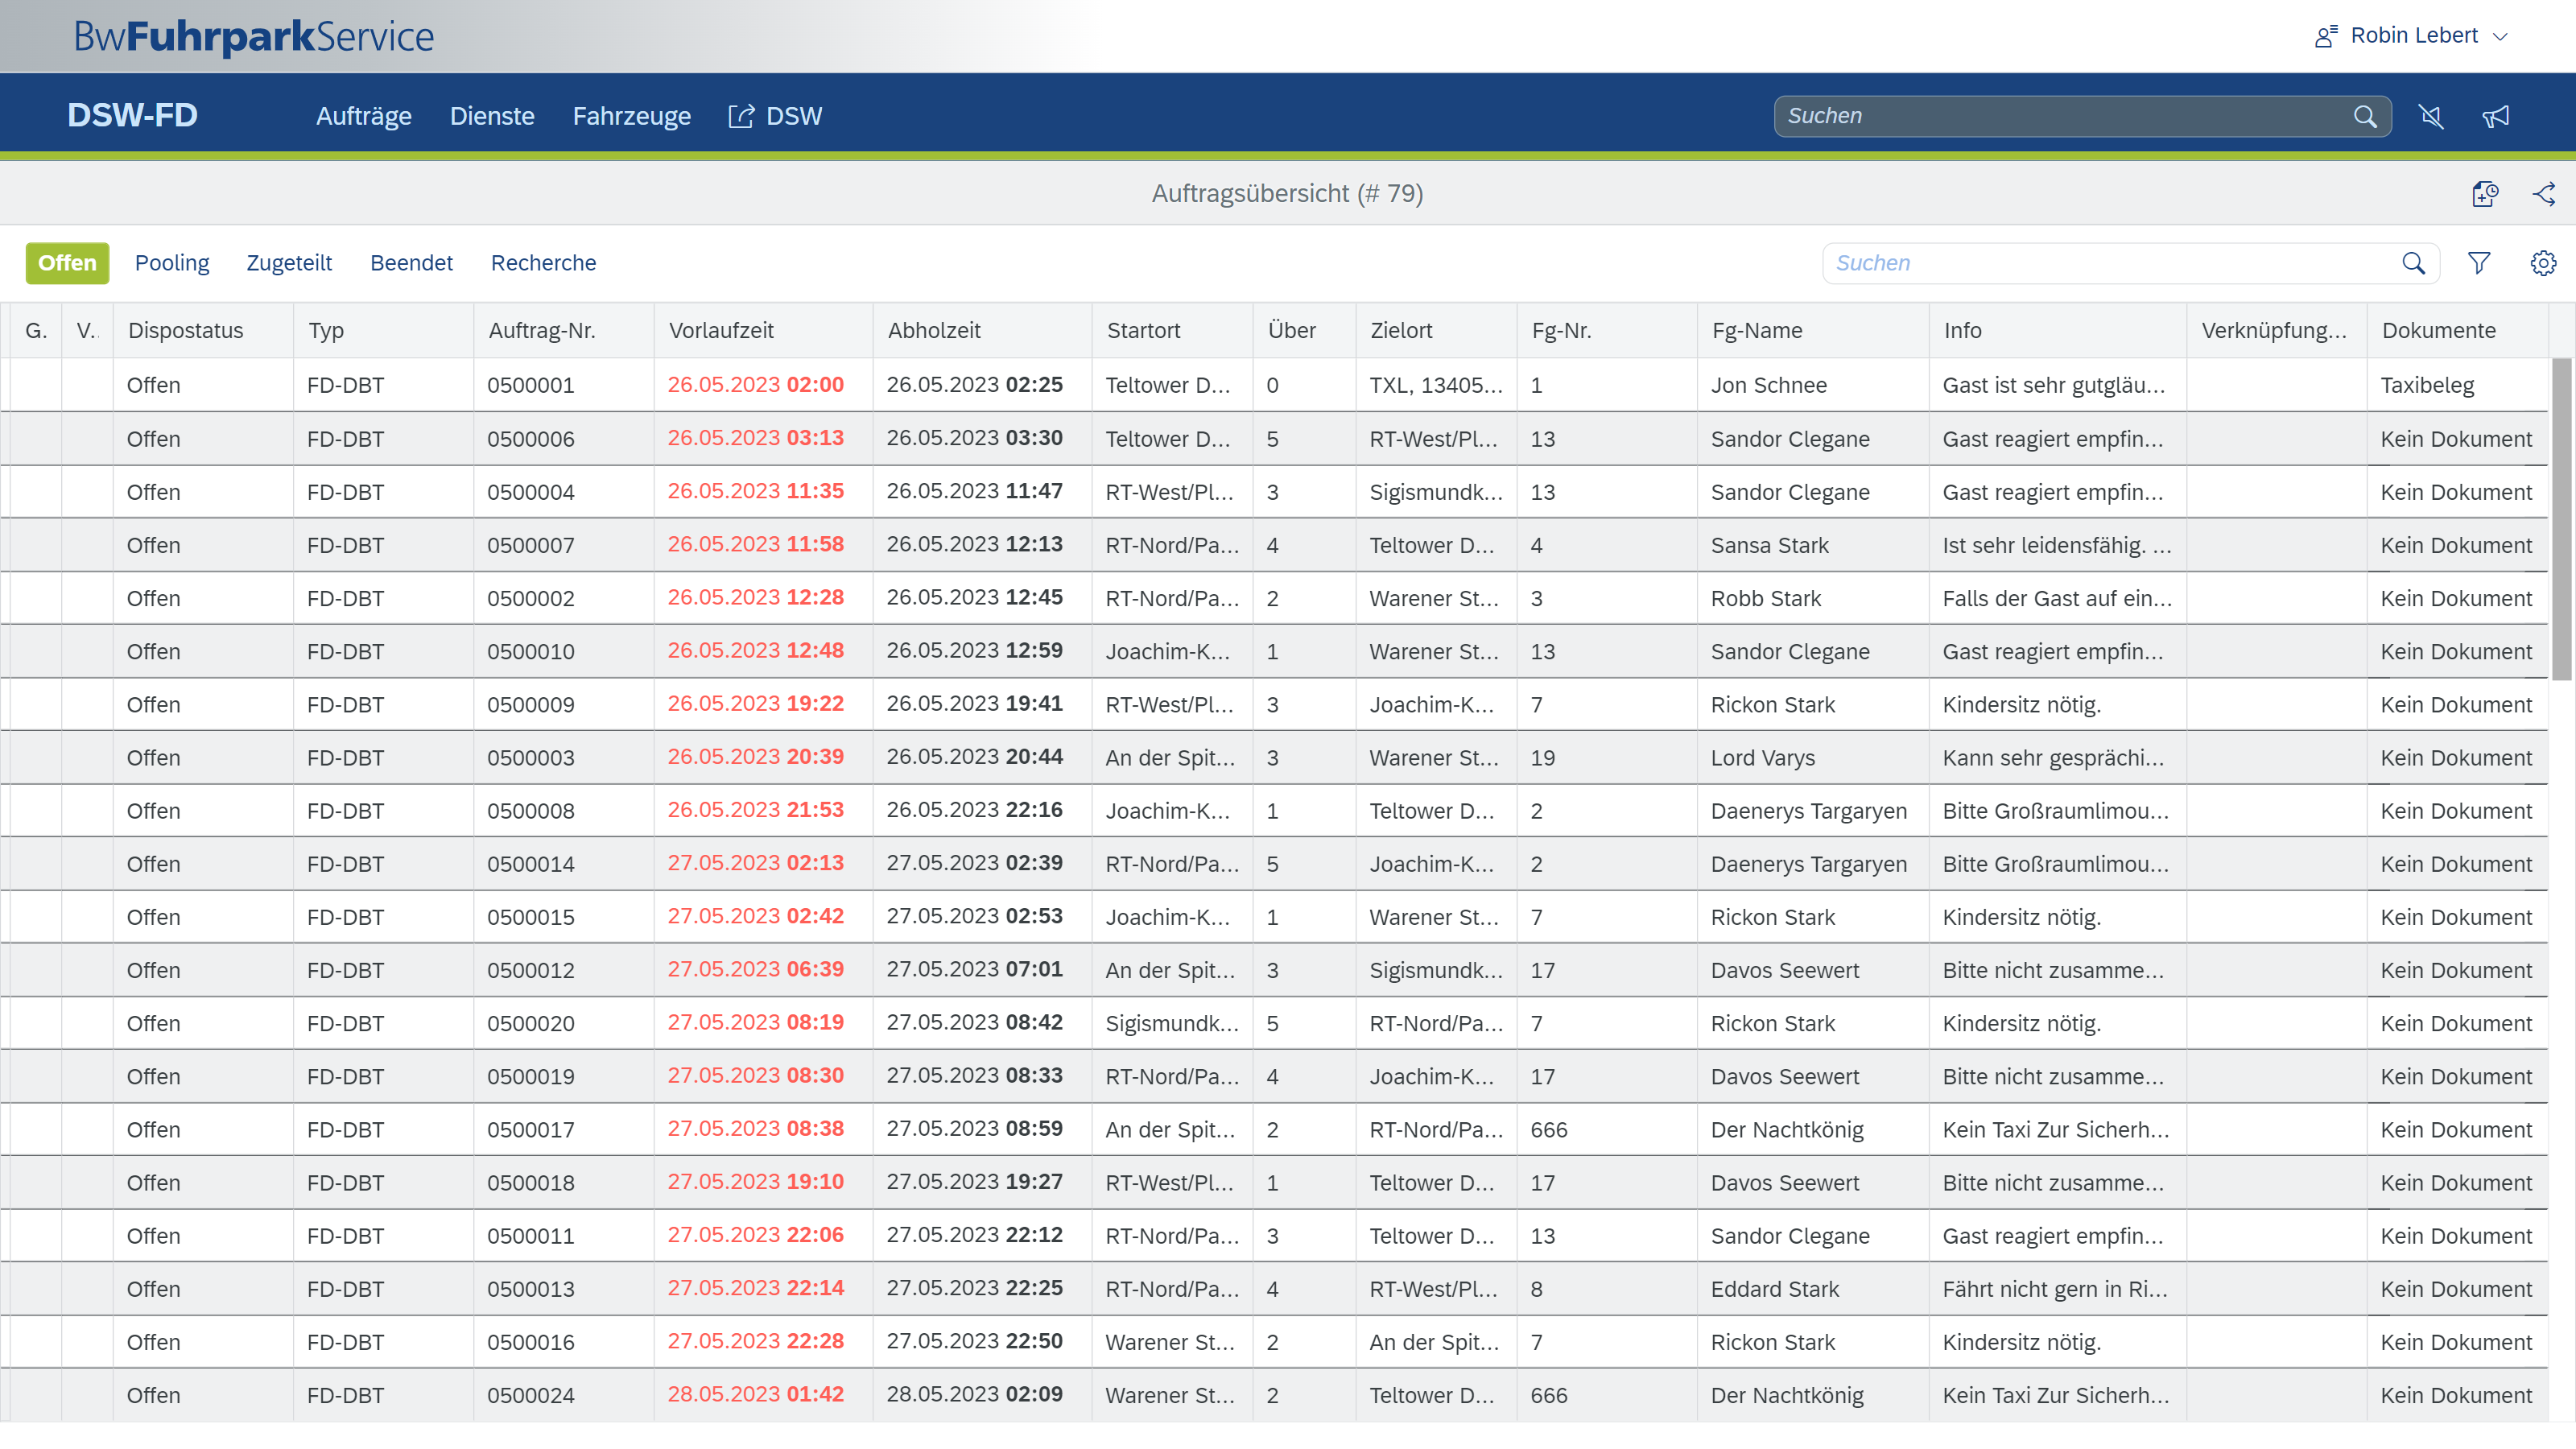
\includegraphics[width=\linewidth]{assets/current-auftrag-overview}
    \caption{Overview of chauffeur jobs in current implementation}
    \label{fig:current-overview-auftrag}
\end{figure}

\begin{figure}
    \centering
    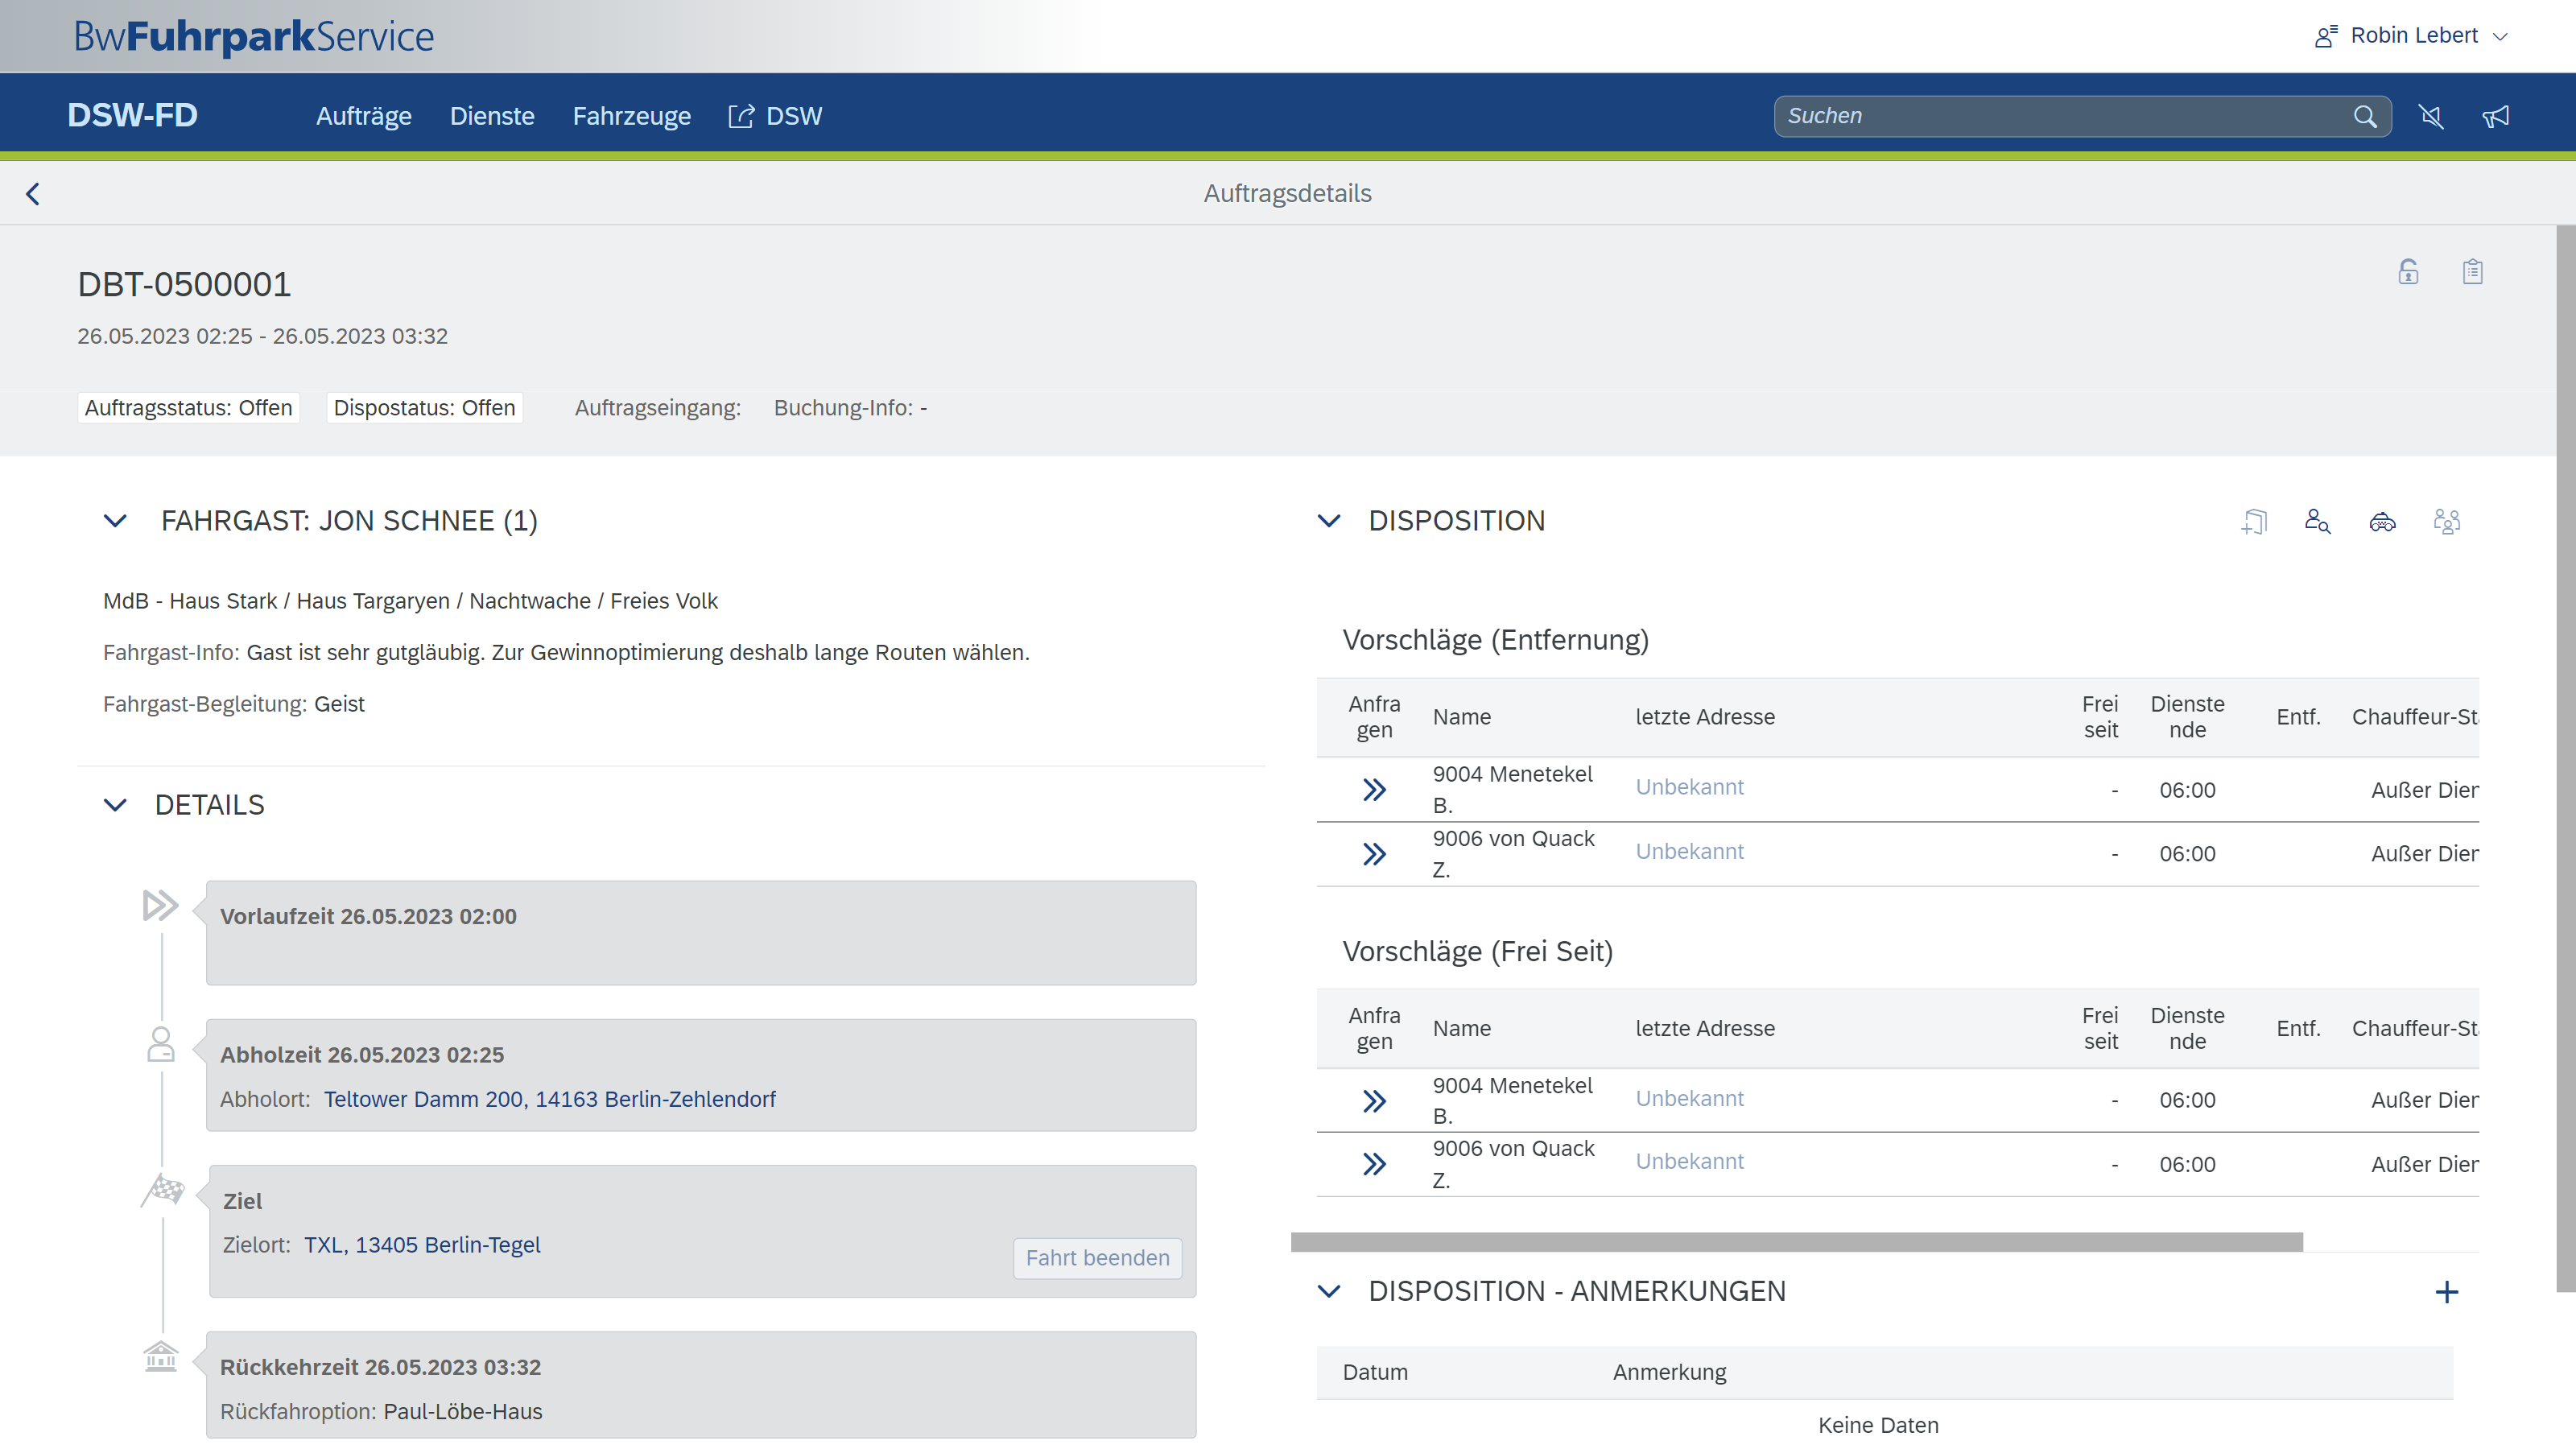
\includegraphics[width=\linewidth]{assets/current-auftrag-details}
    \caption{Chauffeur job details view in current implementation}
    \label{fig:current-details-auftrag}
\end{figure}


\subsection{Full Stack Implementation}

% \begin{itemize}
%     \item prisma 
%     \item easier Authentication
% \end{itemize}
Our first approach was the full stack implementation. This implementation has to replace the UI5 frontend as well as the Spring backend (\Cref{fig:dswfd-architecture-fullstack}). To this end business logic, database communication and API's all have to be implemented in SvelteKit. We used Prisma\footnote{\url{https://www.prisma.io}} for object relational mapping to communicate with the database, because Prisma provides functionality to generate its data model from an existing database using introspection. This allowed us to save time on defining models.

\todo{I feel like this section needs more text}

\begin{figure}
    \centering
    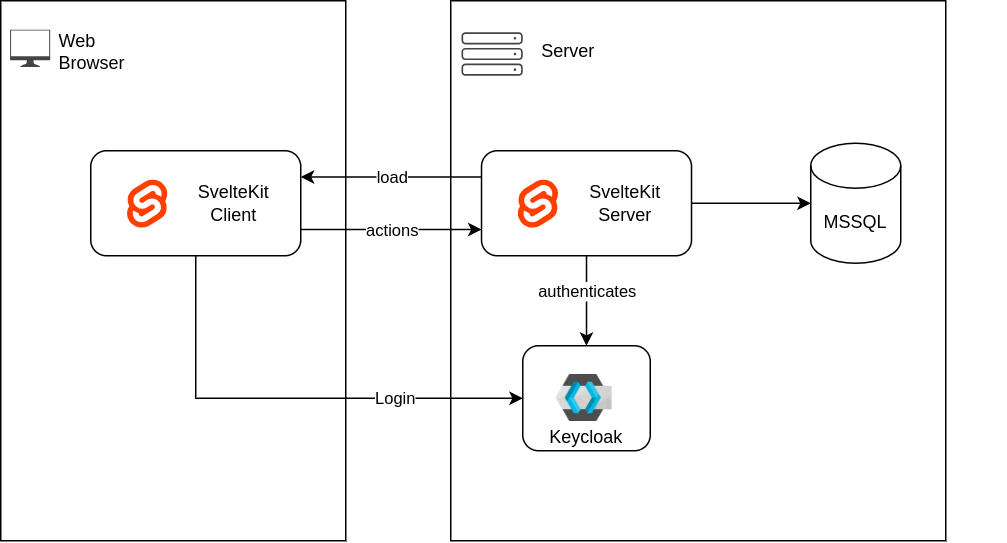
\includegraphics[width=.8\linewidth]{assets/dswfd-architecture-fullstack}
    \caption{Architecture overview of the implementation using SvelteKit as a full stack framework}
    \label{fig:dswfd-architecture-fullstack}
\end{figure}

\subsection{Frontend Implementation}

% \begin{itemize}
%     \item Experimented with direct communication to backend.
%     \item Using universal load functions
%     \item load on server during SSR,
%     \item then client takes over.
%     \item approach would make it possible to run app in SPA mode

%     \item Also tried to route all client requests through SvelteKit backend
%     \item easier because use of locales makes authentication simpler and no problems with custom fetch
%     \item enables usage of form actions, otherwise SvelteKit does not really provide any help with post requests.
% \end{itemize}

We also decided to explore an approach where SvelteKit is only used as a frontend. This approach provides more flexibility, as backend technology can be chosen individually. Communication to the backend is primarily handled using web API's. In our use case we decided to reuse the existing Java backend. The backend's REST API could be queried from SvelteKit. As REST APIs are something which can be called from frontend and backend, this approach can make use of SvelteKit's universal load functions (\Cref{sec:sveltekit-loading}). This means that the SvelteKit server is only used during SSR. After the browser has loaded the page, universal load functions are executed client-side and thus the client directs its requests directly to the backend instead of sending  a request to the SvelteKit server, which then requests the data, from the backend, overall saving one step of indirection. If loss of SSR is acceptable, this approach would also make it possible to run the application as an SPA, forgoing a dedicated SvelteKit server. This can be useful, as it allows for the SvelteKit application to be served as static files from a web directory or similar.

\begin{figure}[ht]
    \centering
    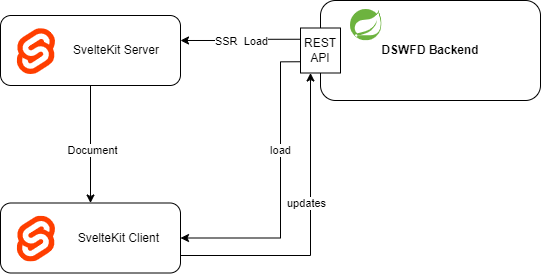
\includegraphics[width=.6\linewidth]{assets/fe-only-client-takes-over}
    \caption{Architecture overview of the implementation using SvelteKit only for the frontend}
    \label{fig:dswfd-architecture-fe-only}
\end{figure}

\subsubsection{Redirect Through Server}
\label{sec:implementation-redirect}

But, this approach has several shortcomings explained in \Cref{sec:evaluation-universal}. Therefore we further experimented with an implementation that again uses server load functions and server actions. This implementation is very similar to the full stack implementation discussed earlier. But instead of implementing business logic and database access in the SvelteKit server side code, the server side is primarily used as middleware that sends REST requests to the Spring backend.

\begin{figure}[ht]
    \centering
    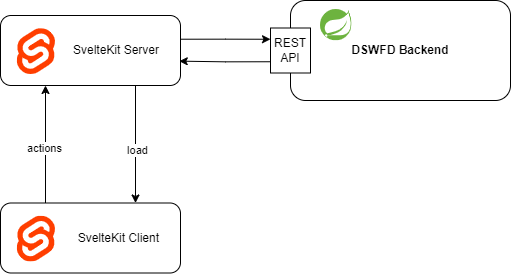
\includegraphics[width=.6\linewidth]{assets/fe-only-all-server}
    \caption{Architecture overview of the implementation using SvelteKit only as a frontend}
    \label{fig:dswfd-architecture-fe-through-server}
\end{figure}

This approach has multiple advantages. It uses much of the built-in functionality of SvelteKit, applications can be progressively enhanced, the client requires fewer dependencies, because functionality such as parsing and validating form data can be handled server side. Furthermore, authentication is simplified, as only the backend needs to communicate with the API. And finally, the outlined problems with fetch in universal load functions is solved, because only the backend uses fetch.


\subsection{UI Considerations}
\label{sec:implementation-ui}

One of the clients requirements for the current implementation was that the frontend follows the SAP Fiori design guidelines. While not strictly necessary for our study, we decided to adhere to this requirement in our SvelteKit implementations. We hoped to gain insights into how SvelteKit behaves, when interacting with UI libraries. The current implementation uses UI5 which has SAP Fiori components built into the framework itself. As it is not possible to use these components outside the framework, we had to use alternatives.   

We first tried to use UI5 Web Components\footnote{\url{https://sap.github.io/ui5-webcomponents/}}. These premade components promise to be a feature rich and framework-agnostic implementation of the Fiori Design Guidelines. In practice, we noticed multiple issues which made use consider alternative solutions. 

\todo{Finish section}

% Our first approach was to use SAP's UI5 Web components. Web components promise to be a framework-agnostic approach to UI components. But we encountered some problems early on:

% \begin{itemize}
%     \item For now, web components can not be server-side rendered. This is because web components rely on API's which only exist in the browser
%     \item Web Components also require JavaScript (at least until \cite{noauthor_declarative_2023})
%     \item Problems: Layout shifting, flash of unstyled content ("FOUC")
% \end{itemize}
